\section*{Definition of Automation Levels for Scientific Discovery}


The AGS concept represents an AI-powered robotic system conceived to conduct research across diverse scientific domains, with the aspiration of matching and eventually exceeding the speed, scope, and depth of human scientists. This section establishes a framework for categorizing AGS into distinct levels based on their degree of autonomy, interaction with both simulated and real-world environments, and overall research capabilities (as detailed in \autoref{tab:ags_levels}). The potential evolutionary trajectory of these levels is illustrated in Figures \ref{ags_timeline} and \ref{ags_evo}.



\subsection*{Level 0: No AI}

At this foundational level, scientific inquiry is executed without the direct involvement of artificial intelligence. Research relies entirely on established methodological approaches and discipline-specific instruments. Scientists utilize specialized equipment and software tailored to particular fields—for instance, spectroscopic devices and analytical platforms in chemistry, or statistical software packages like SPSS and epidemiological modeling tools in public health. While highly effective within their designated areas, these conventional resources typically lack the capacity for seamless interdisciplinary integration and necessitate substantial human expertise for their interpretation and application.



\subsection*{Level 1: Tool-Assisted}

This level marks the introduction of simple AI tools designed to aid researchers in specific, narrowly defined tasks. Primarily driven by human scientists, the AI offers basic functionalities such as API-driven data retrieval, automated text generation, and the identification of simple connections across disciplines. Examples of systems at this level include tools like ChatGPT for text-based assistance and foundational machine learning models for data processing. While the AI can contribute by processing and summarizing information or offering suggestions in response to direct prompts, its capabilities for independent action and initiative remain limited.



\subsection*{Level 2: Intelligent Assistant}

At this stage, AI systems begin to function as sophisticated research assistants capable of navigating and synthesizing knowledge from various domains. Under human supervision, these intelligent agents can autonomously conduct web-based information gathering, perform virtual simulations, and integrate insights from diverse scientific disciplines. Systems such as OpenDevin, DeepResearch, which offer assistance in data acquisition, analysis, and the formulation of hypotheses, are representative of this level. However, significant human oversight is still required to define the scope of their activities and interpret the resulting information.

\subsection*{Level 3: Collaborative Partner}

AI systems at this level evolve into autonomous collaborative partners in scientific research, seamlessly integrating interactions with both virtual and physical environments. Equipped with advanced robotics, they can conduct experiments in domains such as biology, engineering, and medicine, performing precise manipulations in the physical world. These systems are capable of autonomously executing complex, interdisciplinary tasks but still operate in collaboration with human scientists, leveraging their respective strengths. Advanced robotic platforms that combine sensor data processing, semi-autonomous experiment execution, and integrated data analysis are key examples at this level.

\subsection*{Level 4: Autonomous Researcher}

At this stage, AI operates with a significant degree of independence, requiring only minimal human guidance. These systems possess the capacity to conduct advanced research in both simulated and real-world settings, employing autonomous information retrieval and synthesizing knowledge from a wide array of fields. They can generate novel insights and propose innovative solutions by identifying and connecting data points from previously disparate areas of study. Artificial General Intelligence Robots (AGIR) exemplify this category, pushing the boundaries of interdisciplinary research while still benefiting from occasional human oversight or intervention for complex problem-solving or ethical considerations.

\subsection*{Level 5: Pioneer}

The highest level represents fully autonomous systems that surpass human capabilities in scientific research. Termed Artificial SuperIntelligence Robots (ASIR), these systems operate entirely independently across all environments—virtual, physical, and experimental—and are capable of conducting groundbreaking research without any human intervention. They not only synthesize knowledge across disciplines but also innovate and formulate entirely new scientific principles. Their work leads to unprecedented scientific discoveries, positioning them as pioneers at the forefront of AI-driven research. While acknowledging the inherent uncertainties in achieving Level 5 autonomy due to substantial technical, ethical, and practical challenges, this level serves as an ambitious long-term goal for the field, inspiring continued exploration and innovation in autonomous scientific discovery.




\begin{table}[ht]
\vskip 0.2in
\begin{center}
\centerline{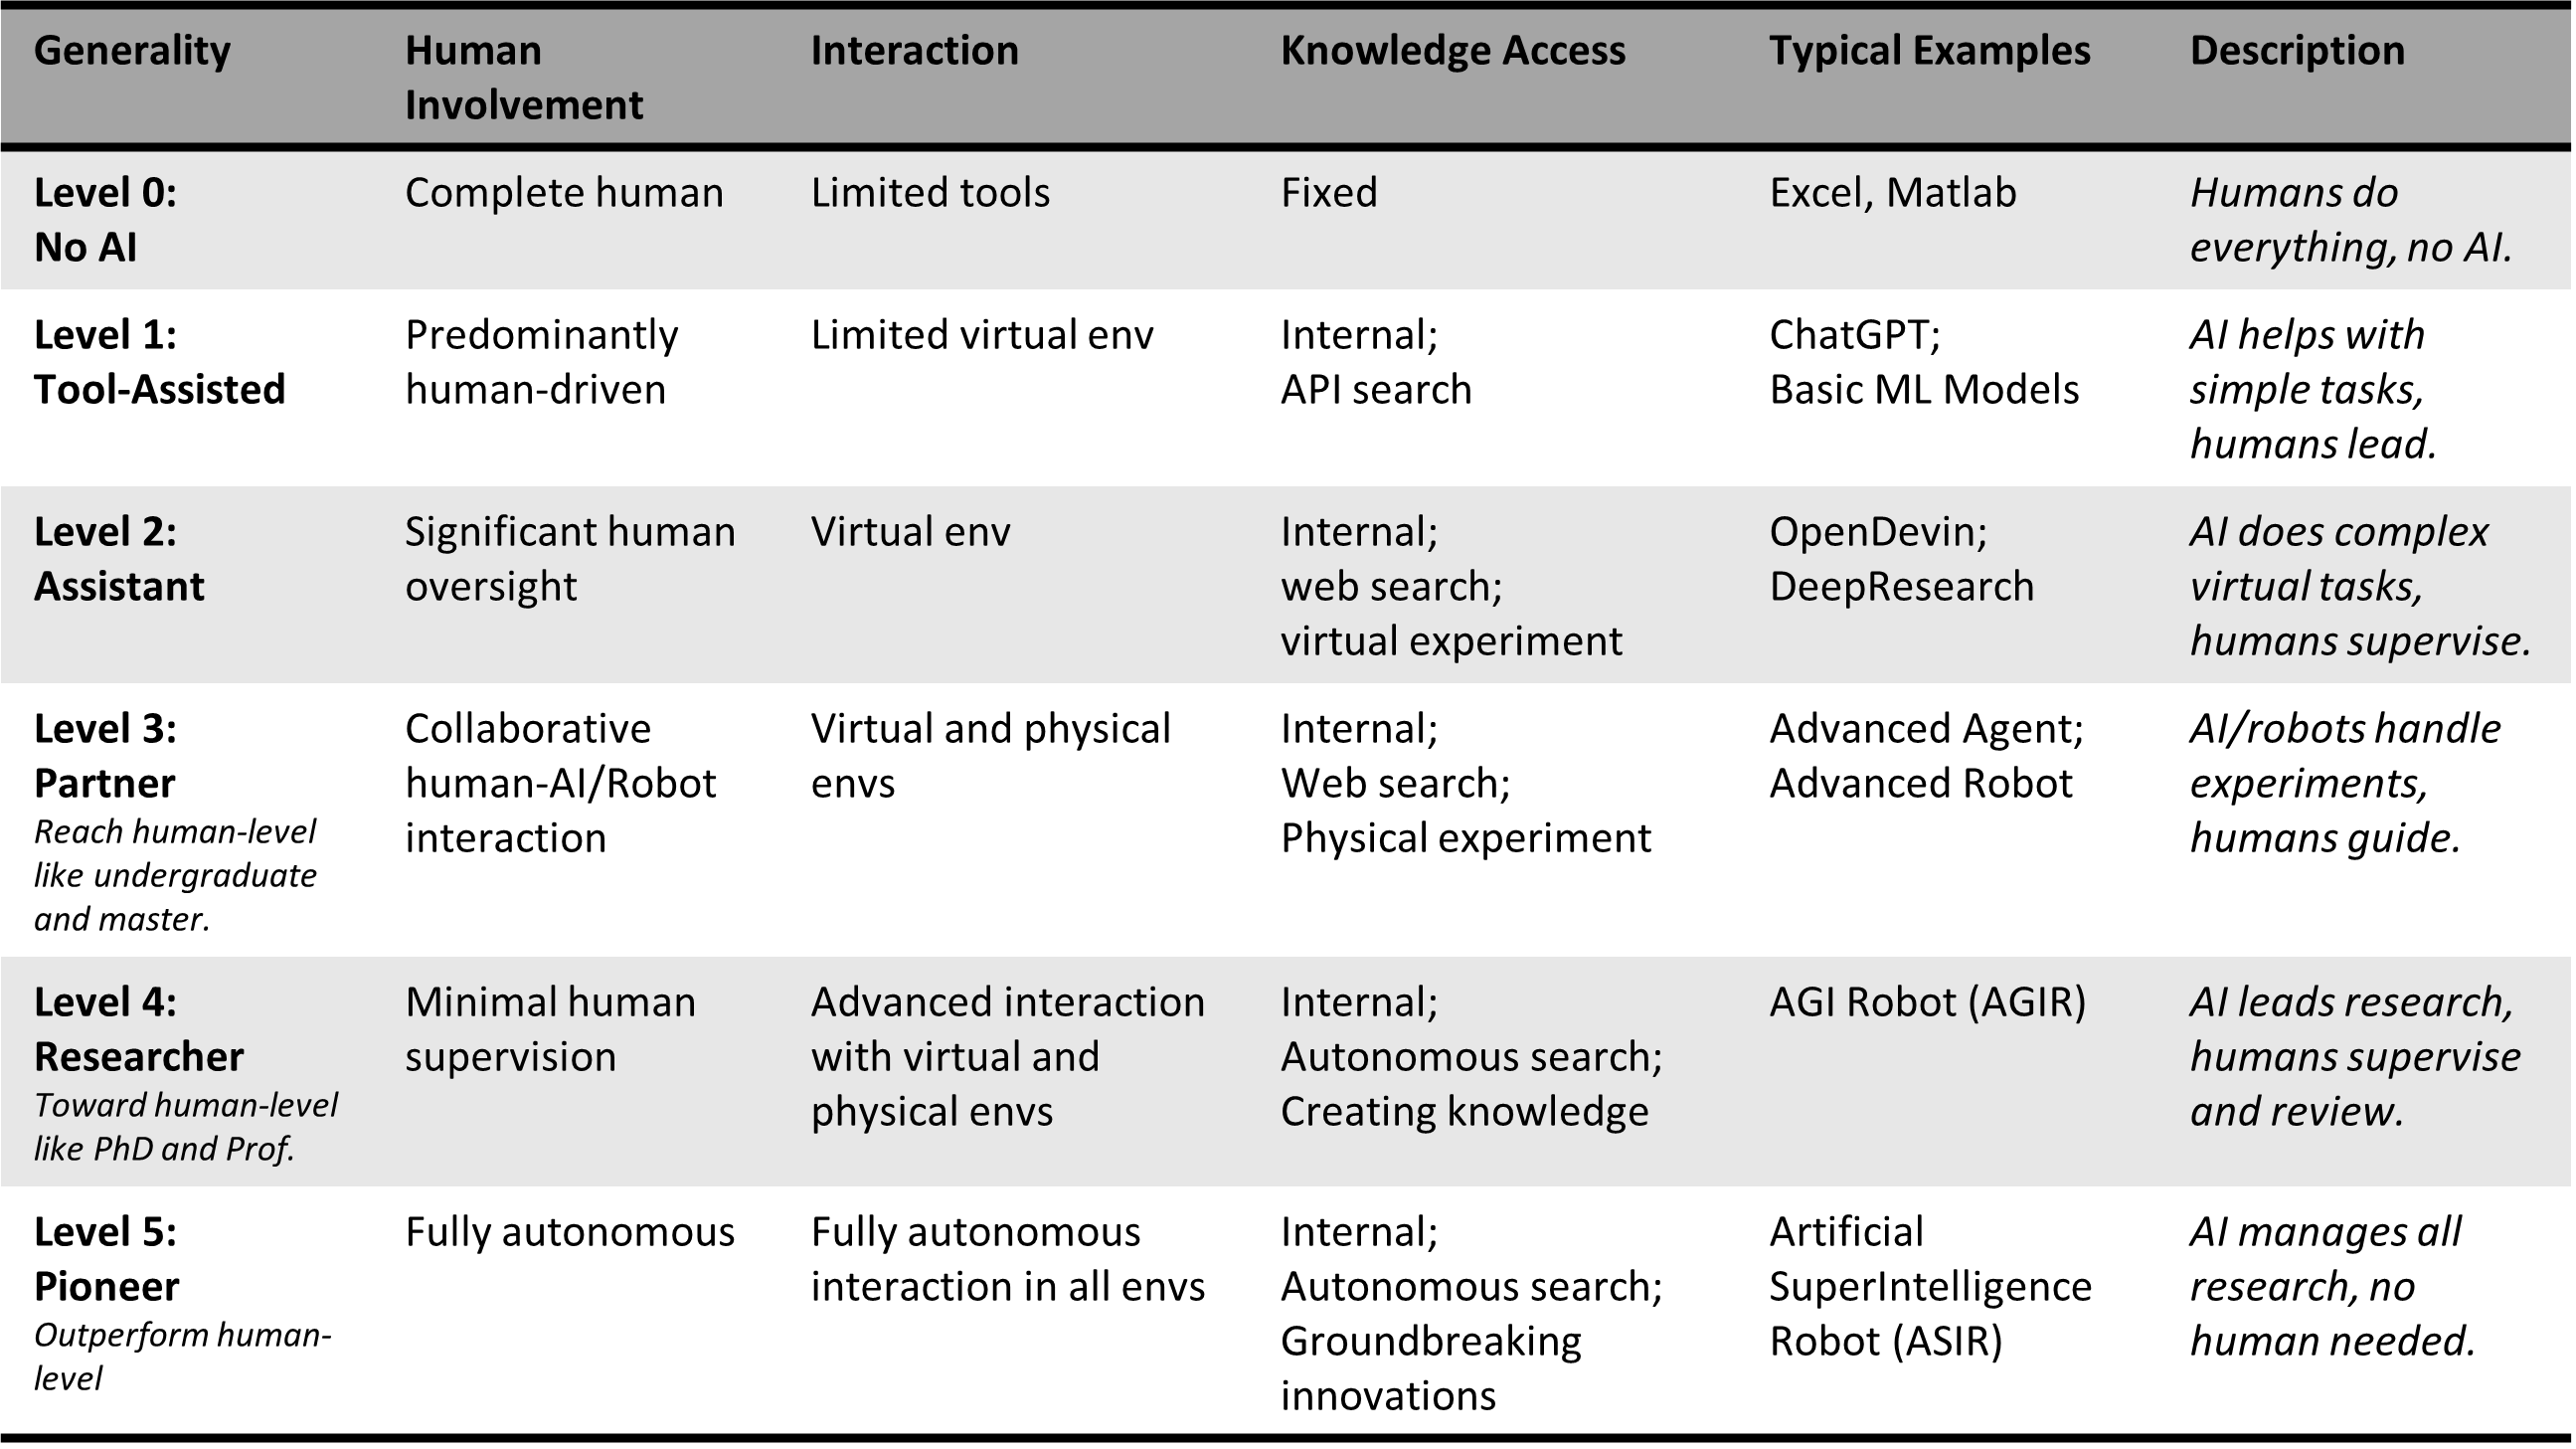
\includegraphics[width=0.99\columnwidth]{resources/figures/levels_table.png}}
\caption{Levels of Autonomous Generalist Scientist.}
\label{tab:ags_levels}
\end{center}
\vskip -0.2in
\end{table}








\begin{figure}[ht]
\vskip 0.2in
\begin{center}
\centerline{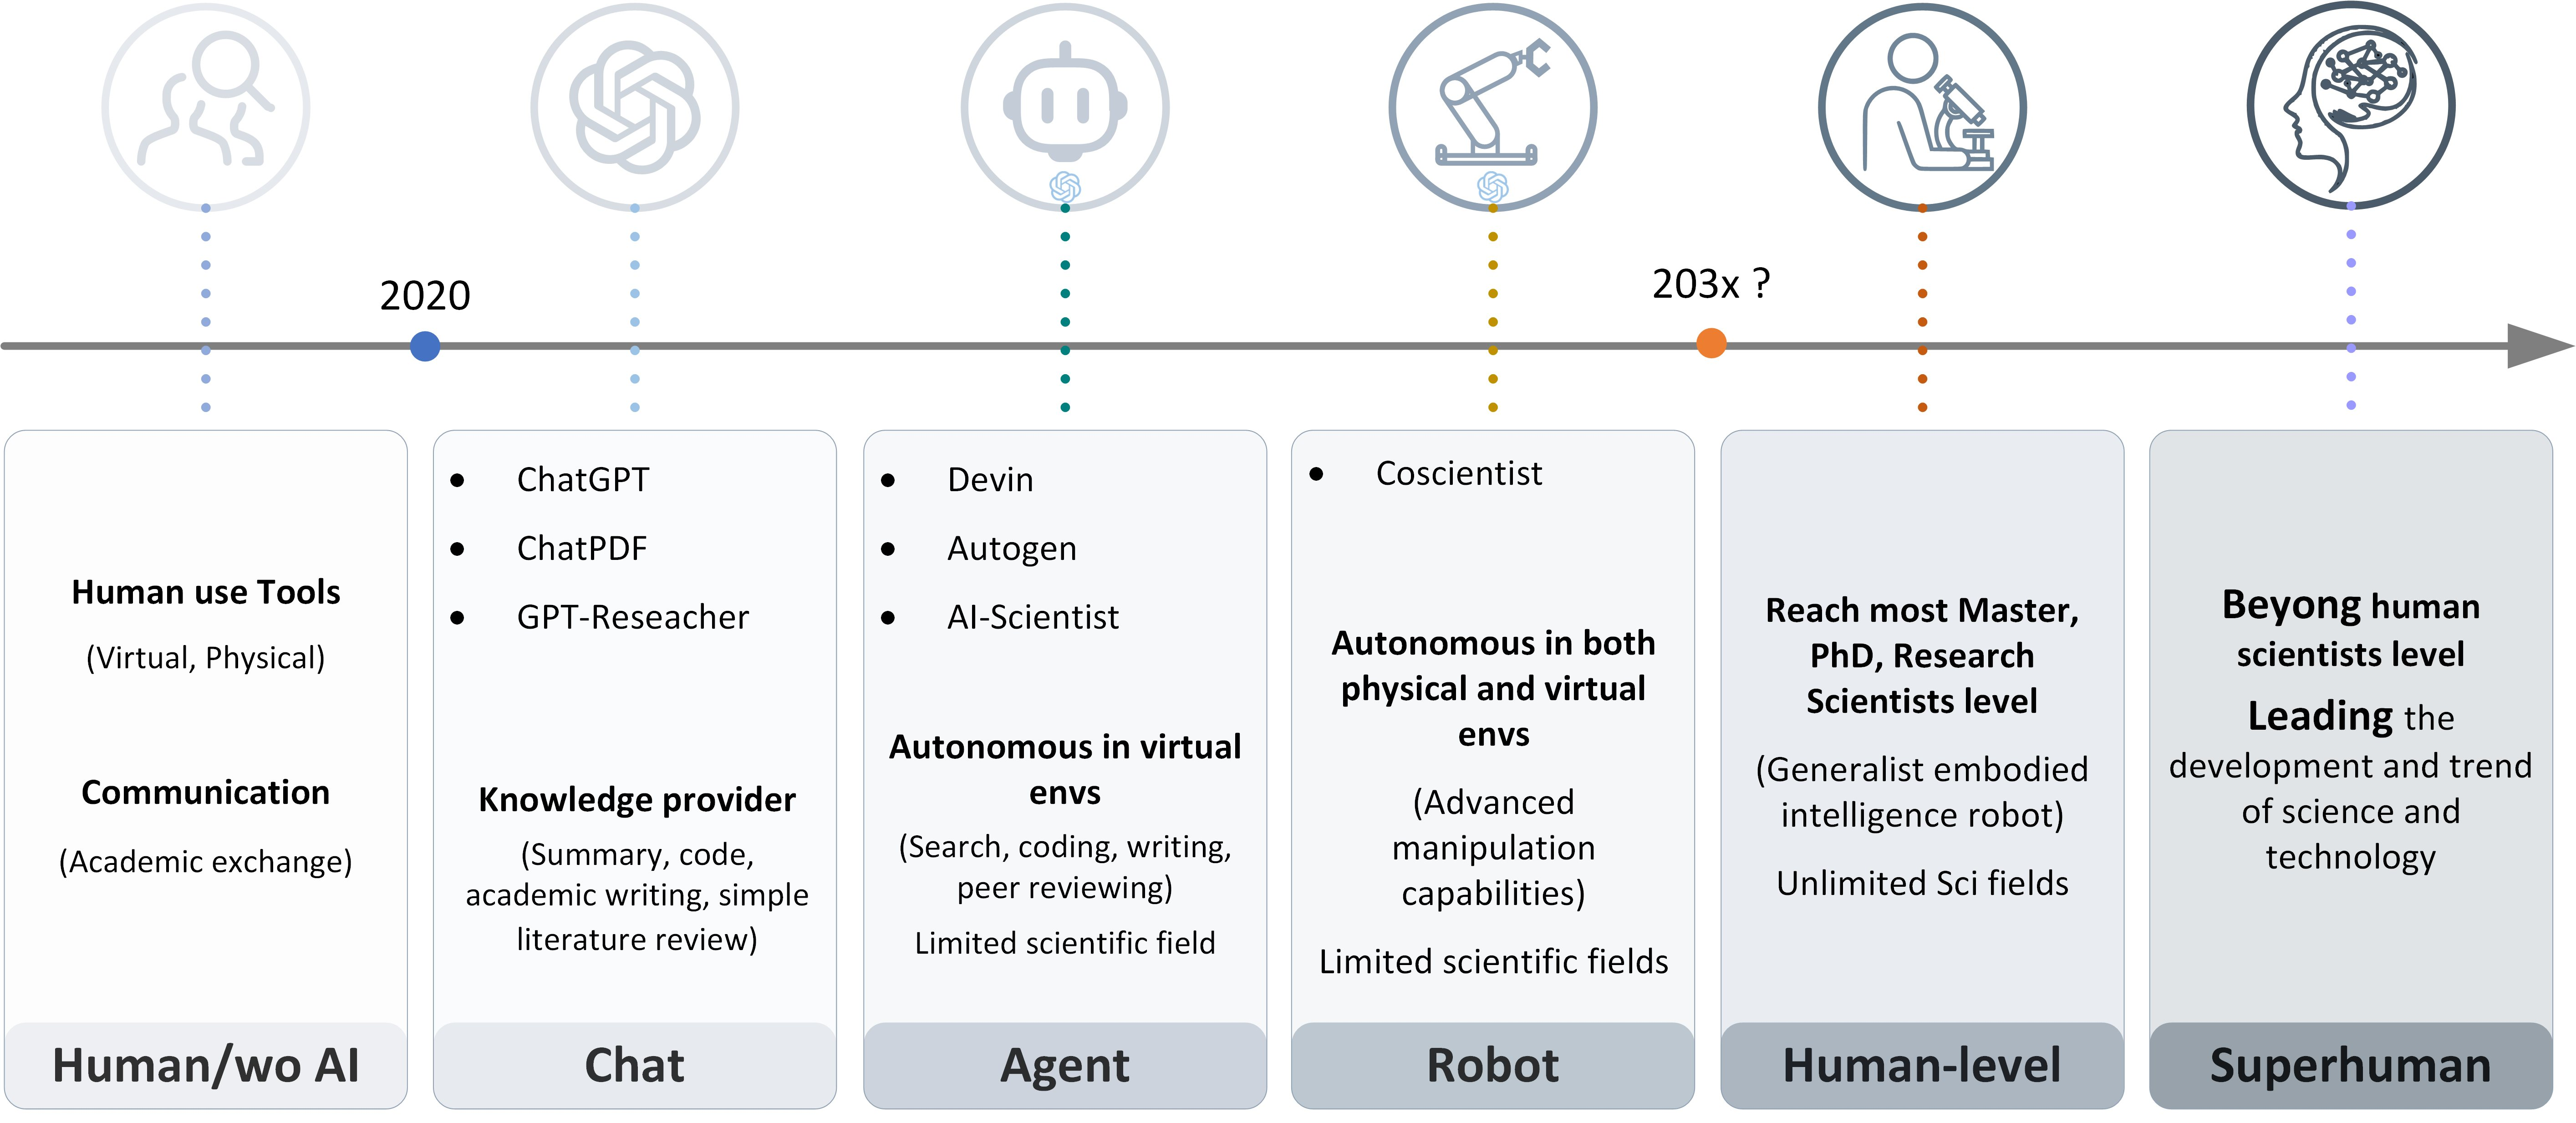
\includegraphics[width=1.00\columnwidth]{resources/figures/ags_timeline.jpg}}
% \caption{Framework of research agents and robots.}
\caption{The timeline of automatic research with different automation levels.}
\label{ags_timeline}
\end{center}
\vskip -0.2in
\end{figure}


\begin{figure}[ht]
\vskip 0.2in
\begin{center}
\centerline{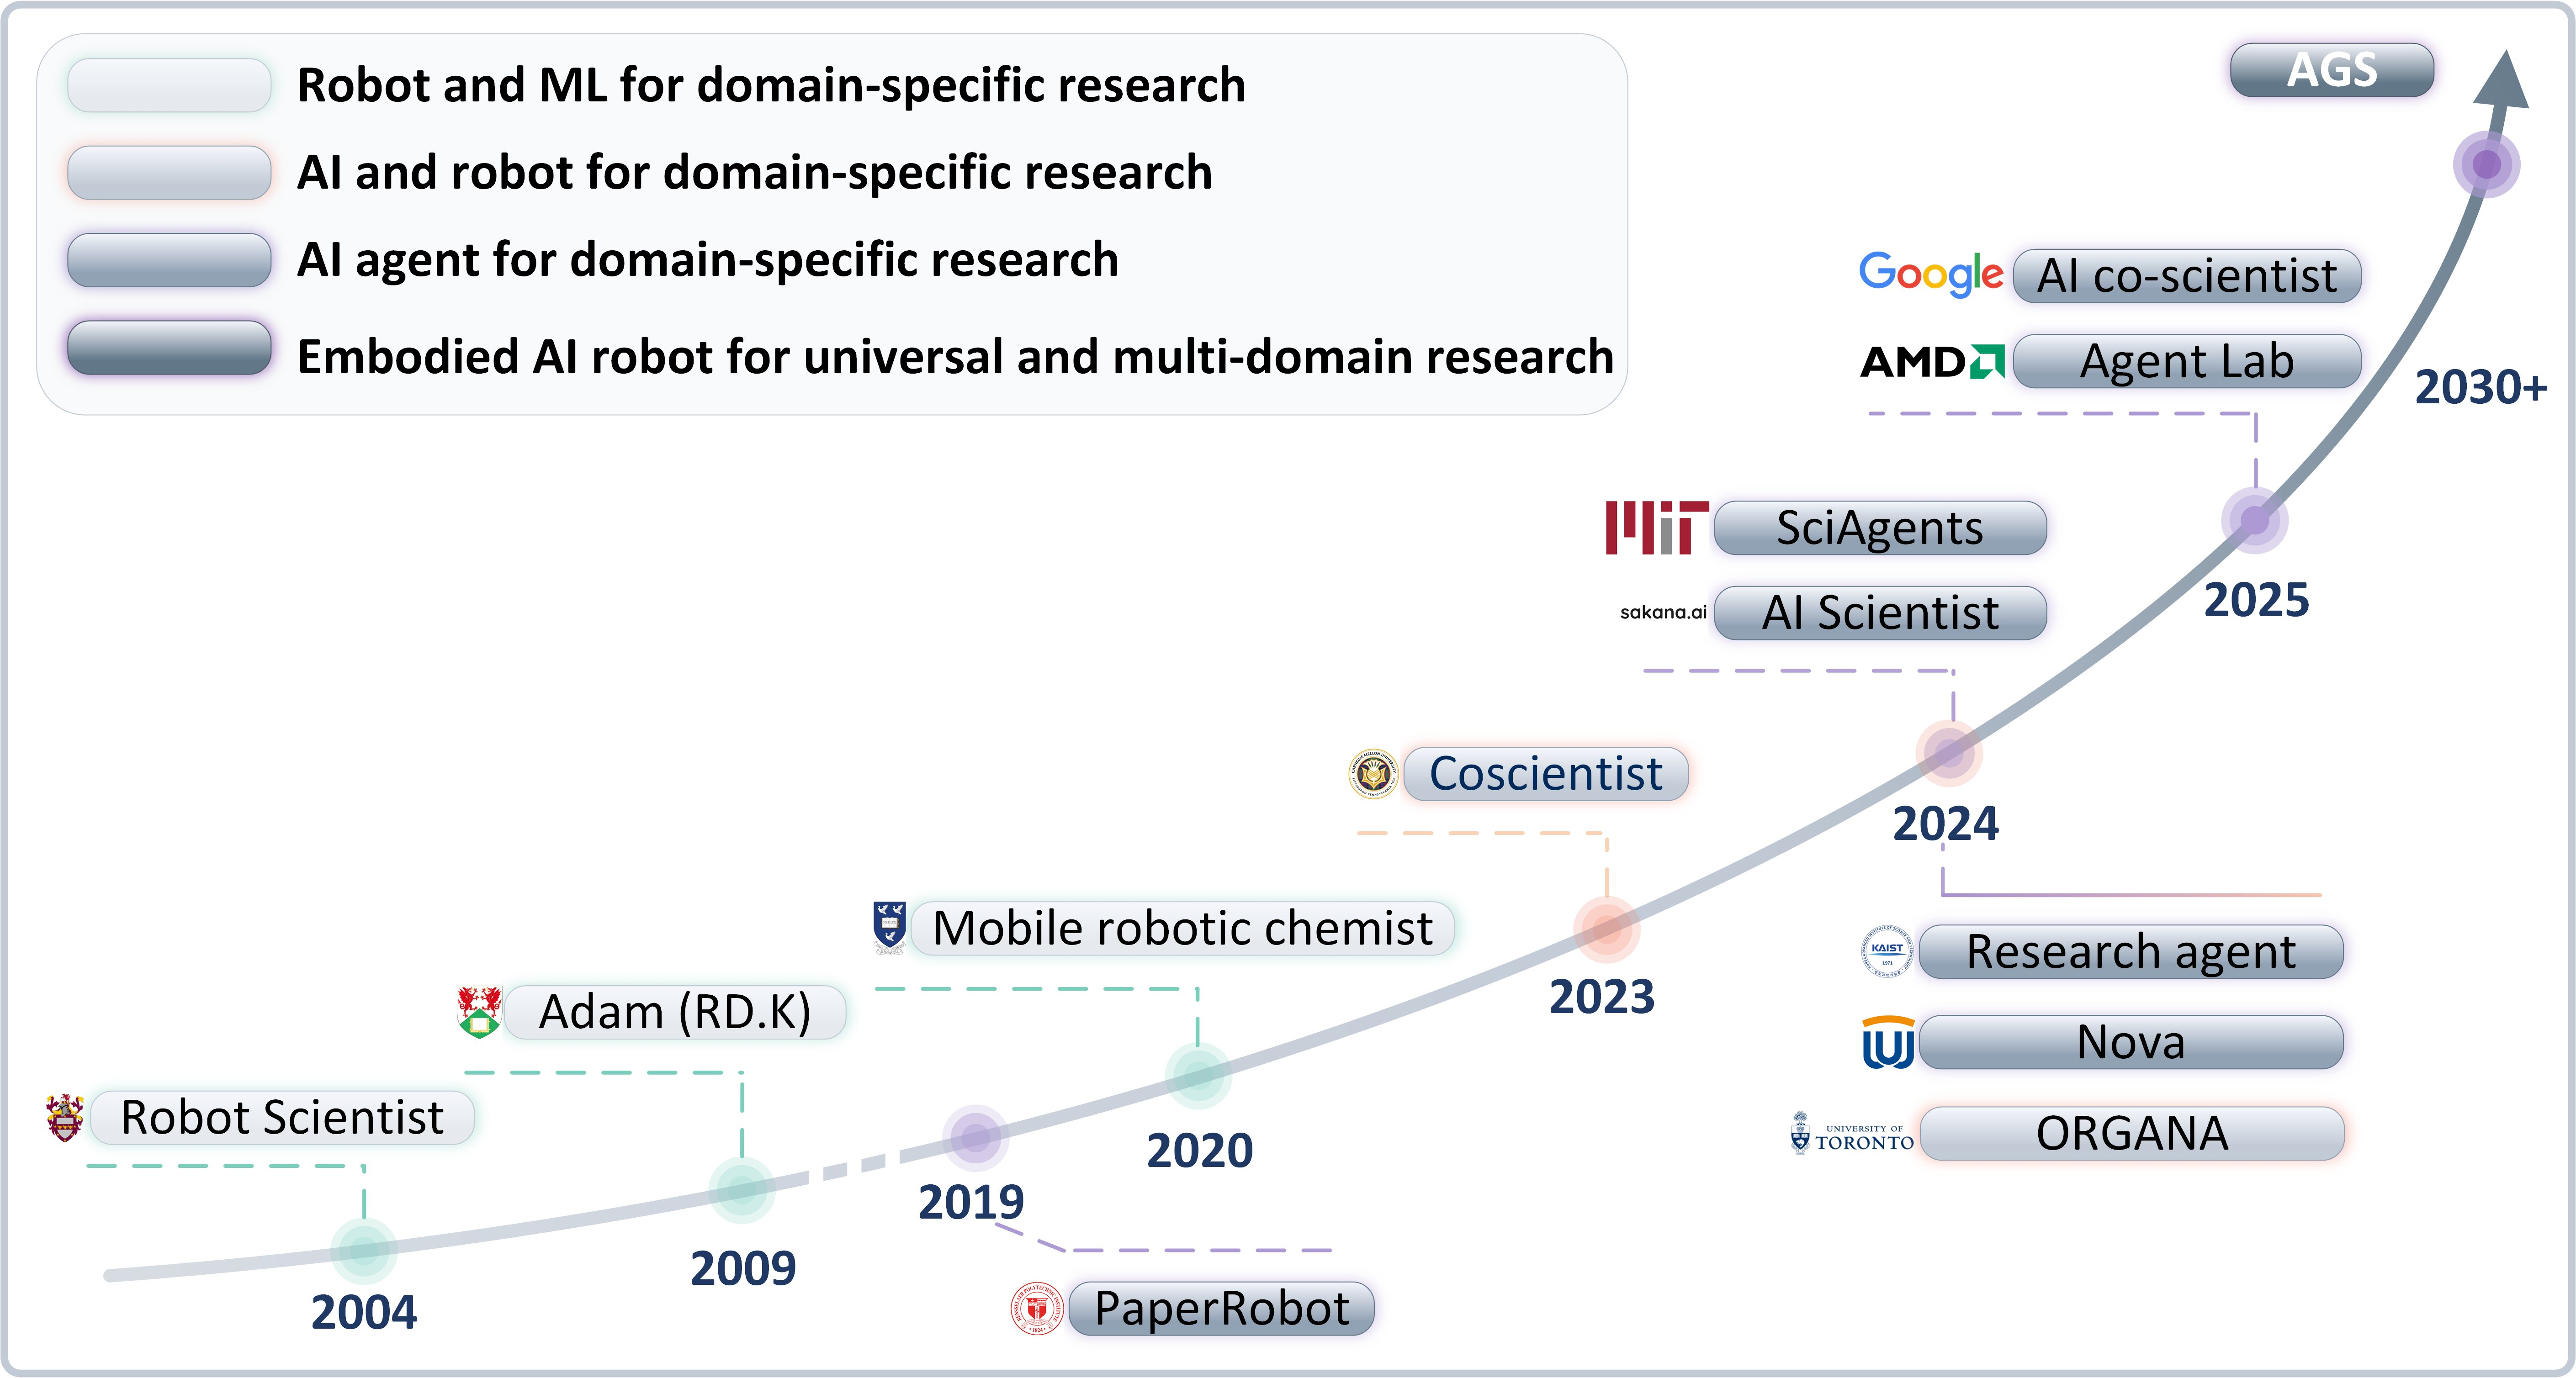
\includegraphics[width=1.00\columnwidth]{resources/figures/ags_evo.jpg}}
% \caption{Framework of research agents and robots.}
\caption{An overview of robot scientist evolution.}
\label{ags_evo}
\end{center}
\vskip -0.2in
\end{figure}



\begin{figure}[ht]
\vskip 0.2in
\begin{center}
\centerline{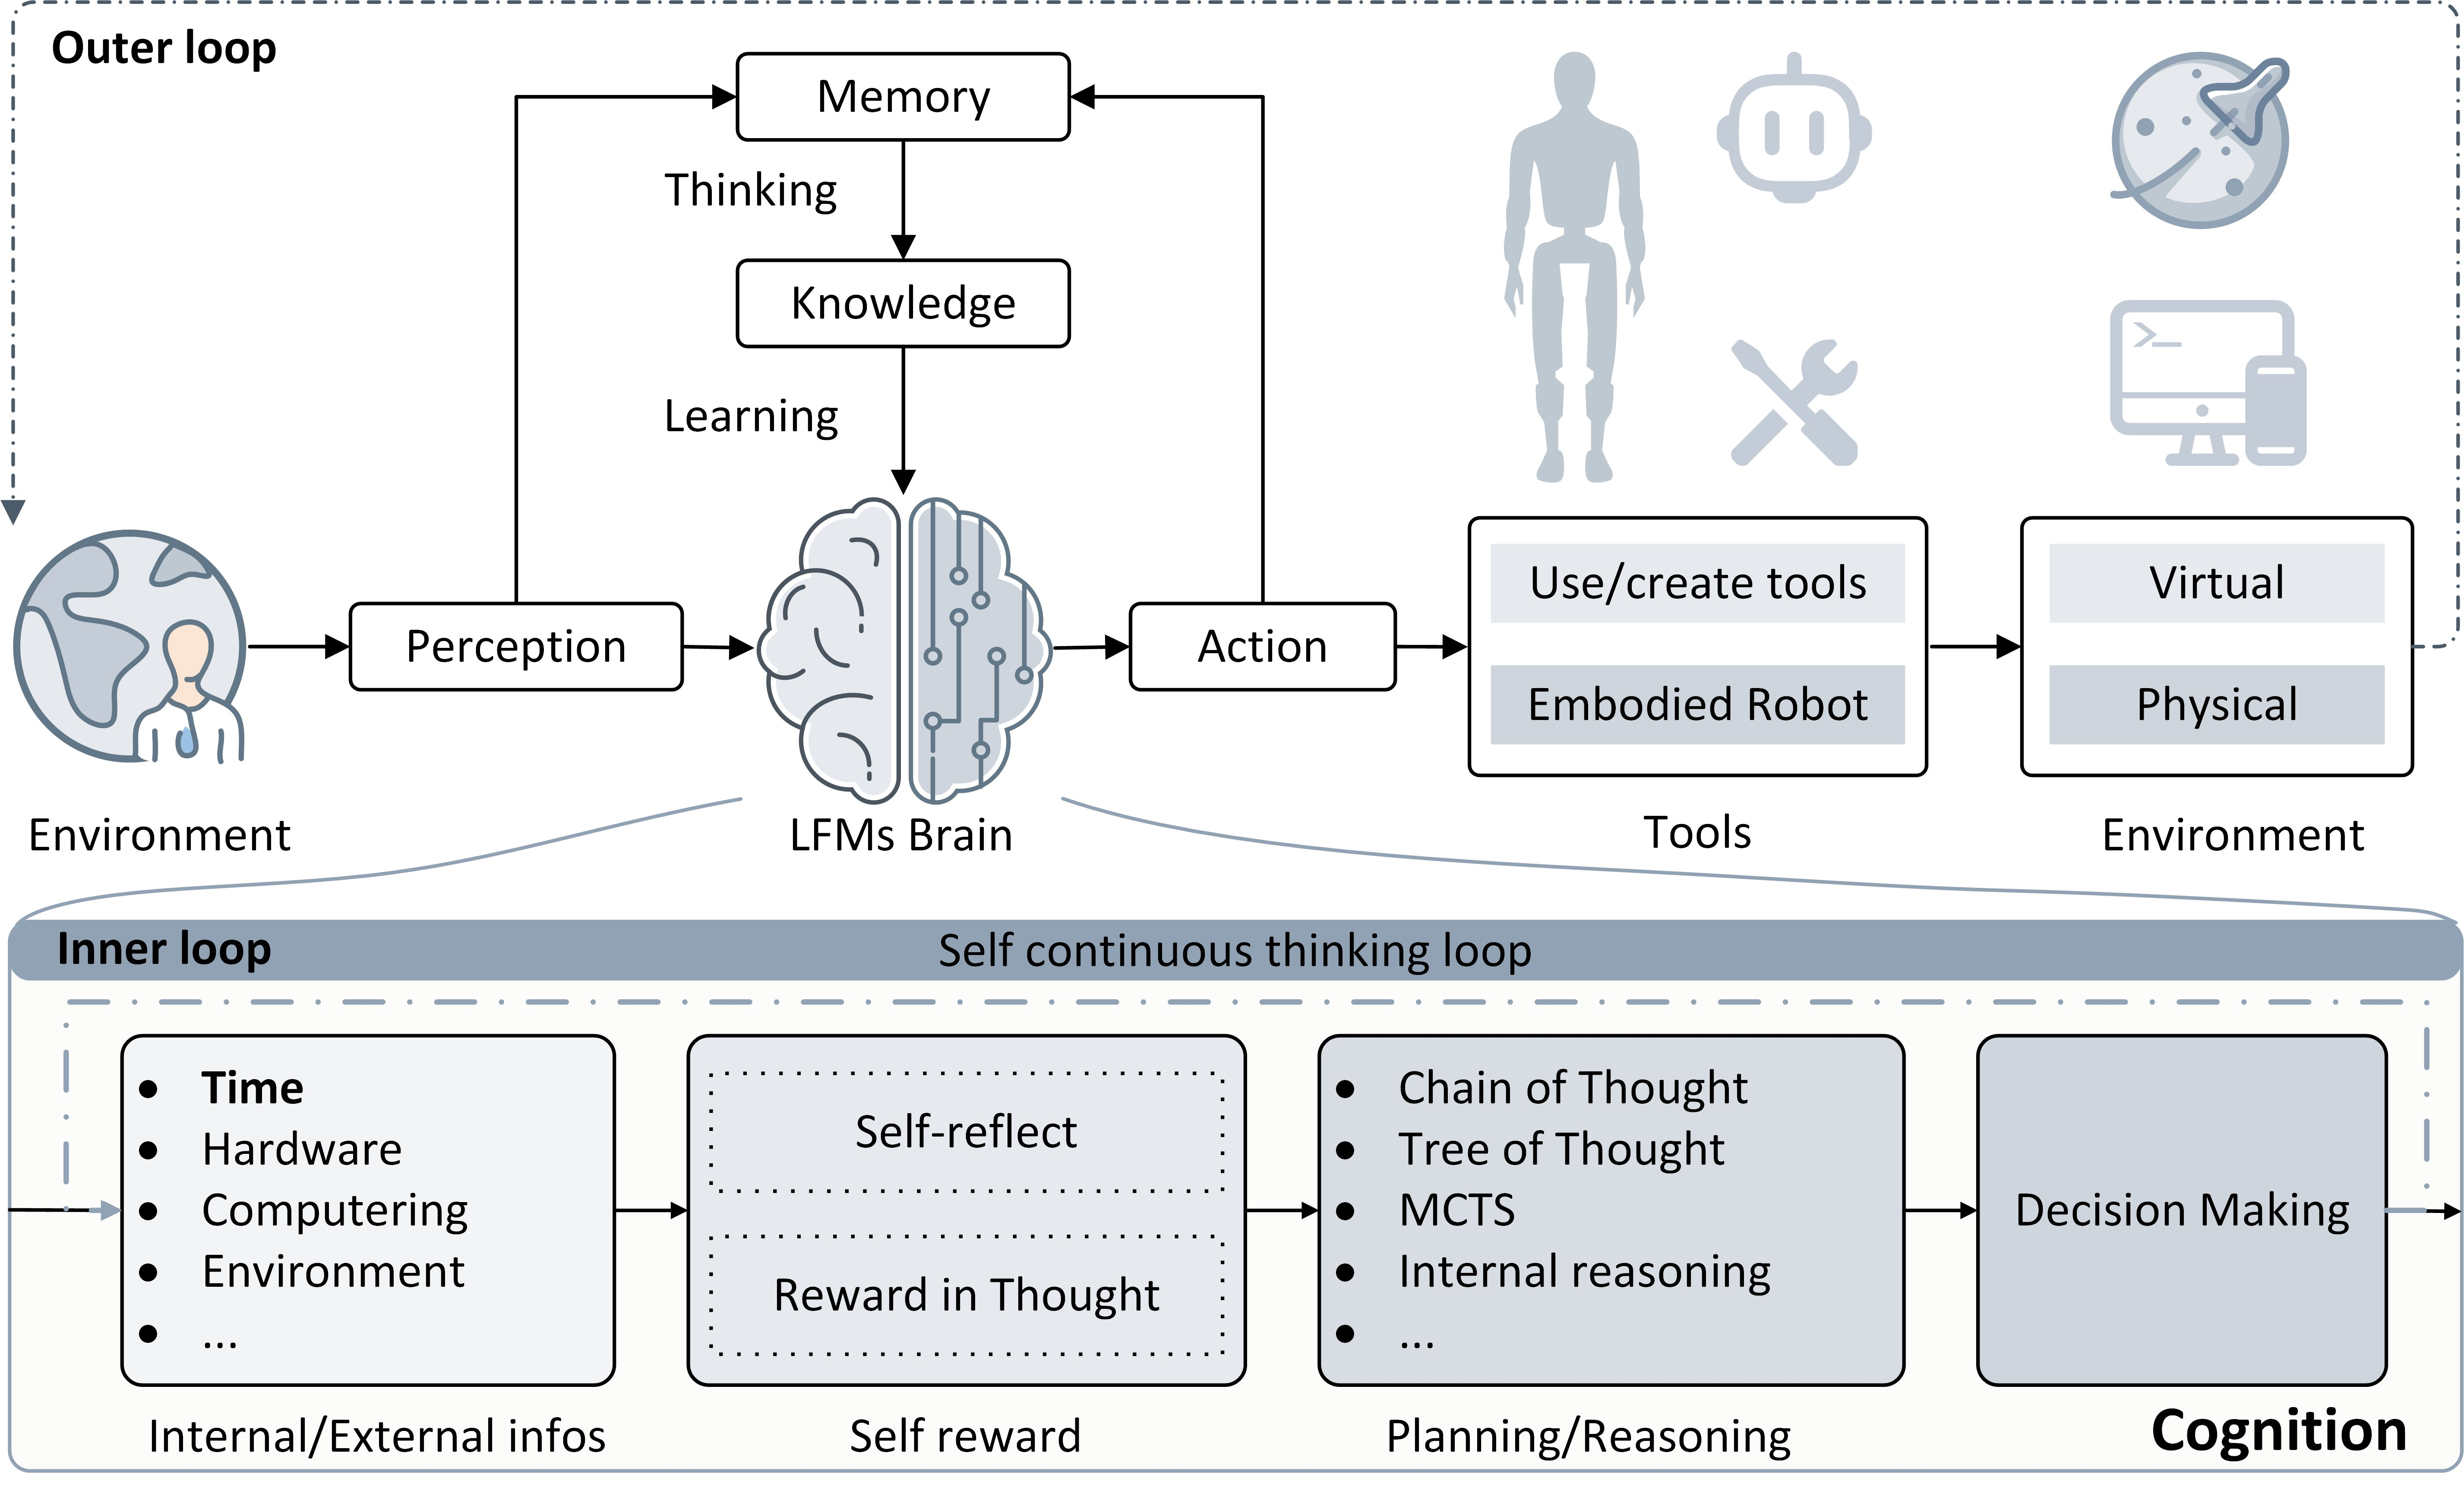
\includegraphics[width=1.00\columnwidth]{resources/figures/ags_brain.jpg}}
% \caption{Framework of AGS brain.}
\caption{Framework of AGS brain.}
\label{ags_brain}
\end{center}
\vskip -0.2in
\end{figure}
